\chapter{Continuous and Discrete-Time Fourier Transform} \label{sec:fourietransforms}
	
	The \de{Fourier transform}, described by the \textit{function} $\F$, is an operator that allows to express a signal $x$ (either continuous depending on the time $t$ or discrete-time depending on the number $n$) in the so called \de{\textit{frequency domain}} ($\Omega$ for continuous-time signals, $\omega$ for discrete-time ones). Such operator can be regarded as the Fourier series, however the difference is that the series operation is performed in the time domain, while the transform operates in the new domain of frequencies.
	
	Given a continuous-time signal $x(t)$ it's \textbf{\ctft} (CTFT) $X(\Omega)$ can be computed as
	\begin{equation} \label{eq:four:ctft}
		X(\Omega) := \int_{-\infty}^{\infty} x(t) e^{-j\Omega t} \, dt \quad \in \mathds C \qquad 
	\end{equation}
	while for discrete-time signals $x(n)$ the definition of the \textbf{\dtft} (DTFT) $X\big(e^{j\omega}\big)$ is
	\begin{equation} \label{eq:four:dtft}
		X\left(e^{j\omega}\right) := \infsum n x(n) e^{-j\omega n} \qquad \in \mathds C
	\end{equation}
	Note that the result of the transform is a complex valued signal, called \de{spectrum}, that can be described by it's \textbf{magnitude} $|X(\Omega)|$ (or $|X(e^{j\omega})|$) and it's \textbf{phase} $\angle X(\Omega)$.
	
	The formal difference between the \textit{continuous frequency} variable $\Omega$ and the \textit{discrete} counterpart $\omega$ lives in their unit of measure: $\Omega$ is in fact expressed as $rad/s$ while $\omega$ is simply expressed as radians. Considering $x(n)$ as a \textit{sampled version} of the signal $x(t)$ with sampling frequency $T_s$, then
	\[ \omega  = \Omega T_s \]
	
	\paragraph{Relationships with other transform} Considering the definition of the Laplace transform
	\[ \mathscr L \big\{ x(t) \} = X(s) := \int_{-\infty}^\infty x(t) e^{-st}\, dt \hspace{2cm} \textrm{with } s = \sigma + j\omega \in \mathds C \]
	that maps a signal into a transfer function in the domain of a complex variable $s$, than it can be observed that the \ctft is the imaginary axis of such plane:
	\[ X(\Omega) = X(s)\Big|_{s=j\Omega} \]
	This means that if a signal has a Laplace transform, then automatically the Fourier one can be determined, while the contrary isn't true  ($x(t)$ can have a Fourier transform but not a Laplace one). Similarly a relation can be seen between the \dtft and the Z transform defined as
	\[ \mathscr Z  \big\{x(n)\big\} = X(z) = \sum_{n=-\infty}^{\infty} x(n) z^{-n}  \hspace{2cm} \textrm{with } z \in \mathds C \]
	In this case the DTFT can be regarded as the evaluation of the Z transform around the unitary circle in the complex plane of the variable $z$:
	\[ X\big(e^{j\omega}\big) = X(z) \Big|_{z=e^{j\omega}}\]
	
	\paragraph{Inverse transform} Every time we have a transform $X$ and important operation that we might want to perform is it's \de{inversion} that allows to reconvert the spectrum into a time-evaluated signal. To perform such operation we can use the formal definition of the \textbf{inverse Fourier transform} that has a slightly difference for continuous and discrete-time original signals:
	\begin{equation} \label{eq:four:inversetransform}
	\begin{aligned}
		x(t) & := \frac 1 {2\pi} \int_{-\infty}^\infty X(\Omega) e^{j\Omega t}\, d\Omega \qquad && \textrm{: continuous-time case} \\
		x(n) & := \frac 1 {2\pi} \int_{-\pi}^\pi X\big(e^{j\omega}\big) e^{j\Omega n}\, d\omega && \textrm{: discrete-time case} 
	\end{aligned}
	\end{equation}
	From this definition is even clearer that, even if $x(n)$ is a discrete-time signal, it's spectrum $X(e^{j\omega})$ is a continuos function; the difference in the inverse Fourier computation between continuous and discrete-time signals is only on the domain on which the integration has to be performed: $[-\infty,\infty]$ in the first case, $[-\pi,\pi]$ in the second.
	
	\paragraph{Existence conditions of the Fourier transform} \label{sec:four:sufficient} In general there's no guarantee that the integral of the Fourier definition converges. No necessary conditions are found in general but we can use a \textbf{sufficient condition} for which {\itshape if a signal $x(t)$ (or $x(n)$) is absolutely summable, then it's transform $X$ exists.} In particular having a absolutely summable signals means that
	\begin{align*}
		& \int_{-\infty}^\infty |x(t)|\, dt < \infty  && \textrm{: continuous-time case} \\
		& \sum_{n=-\infty}^\infty |x(t)|\, dt < \infty \qquad && \textrm{: discrete-time case}
	\end{align*}

	\begin{proof}
		We can use the absolutely summable definition to assert that a spectrum exists considering the following inequalities:
		\[|X(\Omega)| = \left| \int_{-\infty}^\infty x(t) e^{-j\Omega t}\, dt \right| \leq \int_{-\infty}^\infty |x(t)|\, \left|e^{-j\Omega t}\right| \, dt\]
		Having that $|e^{j\Omega t}|$ is always equal to 1, then if the $x$ is infinitely summable than it means that the absolute value of the spectrum must be limited, hence existing.
	\end{proof} \noindent

	While such condition is sufficient to say that a signal surely has a transform, the contrary cannot be said: there are in fact signals that are not absolutely summable but that still presents a Fourier transform.
	
	Considering as example the continuous-time signal $x(t)$ whose spectrum is described by a rectangular distribution $X(\Omega) = \rect_{2\Omega_c} (\Omega)$ (where $\Omega_c = 2\pi f_c$), using the definition of the inverse Fourier transform (equation \ref{eq:four:inversetransform}) we have that
	\begin{align*}
		\antifour{X(\Omega)}(t) & = \frac 1 {2\pi} \int_{-\infty}^\infty X(\Omega) e^{j\Omega t}\, d\Omega = \frac 1 {2\pi} \int_{-\Omega_c}^{\Omega_c} e^{j\Omega t}\, d\Omega \\
		& = \frac{e^{j\Omega_c t} - e^{-j\Omega_c t}}{2\pi j t} = \frac{\sin\big(\Omega_c t\big)}{\pi t} \frac{2f_c}{2f_c} = \frac{\sin\big(2\pi f_c t\big)}{2\pi f_c t} 2f_c  \\ 
		& = 2 f_c \sinc\big(\Omega_c t\big)
	\end{align*}
	Determined $\sinc x = \frac{\sin x}{x}$ the \textbf{cardinal sine} function (whose graph is in figure \ref{fig:four:sinc}), it can be shown that such signal is not absolutely summable, however it's transform exists (and is rectangular).
	
	\begin{SCfigure}[2][bt]
		\centering \includegraphics[width=7cm]{sinc}
		\caption{representation of the cardinal sine $sinc(x)$ function.} \label{fig:four:sinc}
	\end{SCfigure}
	
\section{Property of the transform}
	Doing digital signal processing involves a lot of spectral analysis and so it's important to understand the most useful properties related to the transforms and the transforms of common used functions.
	
		In this section (while not otherwise specified) the reported properties are meant to work on both discrete and continuos-time Fourier transform (while still the proof will be presented for only one type of signal).
		
		\paragraph{Linearity} The Fourier transform is a linear operator, meaning that for every signal $x_1(\cdot),x_2(\cdot)$ that has associated transforms $X_1(\cdot),X_2(\cdot)$ and for every constant coefficient $a,b \in \mathds R$, then 
		\begin{equation}
			\four{ax_1(\cdot) + b x_2(\cdot)} = a \four{x_1(\cdot)} + b\four{x_2(\cdot)} = a X_1(\cdot) + bX_2(\cdot)
		\end{equation}
		
		\begin{proof}
			the proof of such properties strictly depends on the linear property of the integrals; expanding the definition of the Fourier transform for continuous-time signals we have
			\[ \int_{-\infty}^\infty \Big(a x_1 (t) + bx_2(t)\Big) e ^{-j\Omega t} \, dt = a \int_{-\infty}^\infty x_1 (t)  e ^{-j\Omega t} \, dt + b \int_{-\infty}^\infty x_2 (t)  e ^{-j\Omega t} \, dt  \]
		\end{proof}
		
		\paragraph{Time shifting} Given a signal $x(t)$ with transform $X(\Omega)$ that's \textit{shifted in time} by a value $t_0$ determining the signal $x(t-t_0)$, then the spectrum of the shifted signal is
		\begin{equation} \label{eq:four:timeshifting}
			\four{x(t-t_0)} = e^{-j\Omega t_0} \four{x(t)} = e^{-j\Omega t_0} X(\Omega)
		\end{equation}
		
		\paragraph{Convolution operator and property} As it will be explained, the behaviour of the output of the system can be regarded as the \textit{convolution} of the input and the impulse response. We so define the \textbf{convolution} operation $x(t)*h(t)$ between the continuous-time signals $x,h$ as 
		\begin{equation}
			y(t) = x(t) * h(t) := \int_{-\infty}^\infty x(\tau) h(t-\tau)\, d\tau
		\end{equation}
		For discrete-time evaluated signals the discrete counterpart of the convolution is defined as
		\begin{equation}
			y(n) = x(n) * h(n) := \sum_{u=-\infty}^\infty x(u) h(t-u)\, du
		\end{equation}
		This operation is commutative, meaning that $x(\cdot)*h(\cdot) = h(\cdot)*x(\cdot)$ and so, while computing the convolution, we can choose the \textit{easier} formulation that simplify the calculations.
	
		With that said the \textbf{convolution property} allows to related the convolution of signals in the time domain as the product of their transforms:
		\begin{equation} \label{eq:four:convolution}
			\four{x(t)*h(t)} = \four{x(t)} \four{h(t)} = X(\Omega) H(\Omega)
		\end{equation}
		
		\begin{proof}
			also in this case the proof can be made by expliciting the definition of the Fourier transform and using properties of the integral calculations:
			\begin{align*}
				\four{x(t) * h(t)} & = \int_{-\infty}^\infty \left( \int_{-\infty}^\infty x(\tau) h(t-\tau)\, d\tau \right) e^{-j\Omega t} \, dt \\
				& =  \int_{-\infty}^\infty x(\tau) e^{-j\Omega \tau} \underbrace{\left( \int_{-\infty}^\infty h(t-\tau) e^{-j\Omega(t-\tau)} \, dt \right)}_{=\four{h(t)}} \, d\tau \\
				& = H(\Omega) \int_{-\infty}^\infty x(\tau) e^{-j\Omega \tau} \, d\tau = X(\Omega) H(\Omega)
			\end{align*}
		\end{proof}
	
		\paragraph{Differentiation in the frequency domain} Another relevant property is related to the differentiation in the frequency domain; given a signal $x(t)$ (but similarly it work for the discrete-time case) with transform $X(\Omega)$ then
		\begin{equation} \label{eq:four:differentiation}
			\four{t\,x(t)} = j \frac{dX(\Omega)}{d\Omega}
		\end{equation}
	
		\begin{proof}
			such property can be proven considering a discrete-time signal $x(n)$; by applying the definition of the \dtft on equation \ref{eq:four:differentiation} we have
			\begin{align*}
				\sum_{n=-\infty}^\infty n x(n) e^{-j\omega n} & = \frac{-j}{-j}\sum_{n=-\infty}^\infty x x(n) e^{-j\omega n}  = j \sum_{n=-\infty}^\infty x(n) \frac{d}{d\omega} \Big(e^{-j\omega n}\Big) \\
				& = j \frac{d}{d\omega}\sum_{n=-\infty}^\infty x(n) e^{-j\omega n} = j \frac{dX(e^{j\omega})}{d\omega}
			\end{align*}
		\end{proof}
		
		\paragraph{Symmetries} Some notable symmetries can be notices while dealing with real evaluated signals $x(\cdot)\in \mathds R$: the transform of such signals are in fact in the form
		\begin{equation}
			X(-\Omega) = X^*(\Omega) \hspace{3cm} X\big(e^{-j\omega}\big) = X^*\big(e^{j\omega}\big)
		\end{equation}
		where $X^*$ is the complex conjugated of $X$.
		\begin{proof} 
			the proof for continuous-time real evaluated signal $x(t)$ can be performed considering the definition
			\begin{align*}
				X(-\Omega) & = \int_{-\infty}^\infty x(t) e^{-j (-\Omega) t} \, dt = \int_{-\infty}^\infty x(t) \left(e^{-j\Omega t}\right)^* \, dt \\ 
				& = \left( \int_{-\infty}^\infty x(t) e^{-j\Omega t} \, dt\right)^* = X^*(t)
			\end{align*}
		\end{proof} \noindent
		
		From this fact we can observe that the \textbf{magnitude spectrum} $|X(\cdot)|$ is always an \textbf{even} function while the \textbf{phase spectrum} $\angle X(\cdot)$ is always \textbf{odd}. From that we can further say:
		\begin{itemize}
			\item if $x(\cdot)$ is real-evaluated and present an event symmetry, then $X(-\Omega) = X(\Omega)$ and the transform is purely real evaluated;
			
			\item if $x(\cdot)$ is real-evaluated and present an odd symmetry, then the complex spectrum $X(\Omega)$ is purely imaginary.
		\end{itemize}
		
		Considering so that every real signal $x(\cdot)$ can be rewritten as the sum $x_e(\cdot) + x_o(\cdot)$ of the following even and odd functions
		\[ x_e(t) = \frac{x(t) + x(-t)}{2} \hspace{3cm} x_o(t) = \frac{x(t) - x(-t)}{2} \]
		then it means that the related spectrum (considering the linearity property) can also be decomposed into a purely real component and an imaginary one:
		\[ X(\Omega) = \int_{-\infty}^\infty x_e(t) \cos(\Omega t) \, dt + j \int_{-\infty}^\infty x_o(t)\, \sin(\Omega t)\, dt = X_e(\Omega) - j X_o(\Omega)\]
		where the results have been obtained using Euler's formula $e^{j\theta} = \cos\theta + j \sin\theta$.
		
		\paragraph{Time reversal} Another property that can be useful is the one that allows to compute the transform of a signal reversed in time; in particular we have that
		\begin{equation}
			\four{x(-t)} = X^*(-\Omega) \hspace{1.5cm} \textrm{and} \hspace{1.5cm} \four{x(-n)} = X^*\big(e^{-j\omega}\big)
		\end{equation}
		
		\begin{note}
			If we also consider that a signal $x(t)$ is real evaluated, using the symmetries relations previously discovered we have that $\four{x(-t)} = X^*(\Omega)$.
		\end{note}
	
	\subsection{Windowing theorem} 
		Assuming to have two signals $x(\cdot),w(\cdot)$  producing the signal $y(t) = x(t) w(t)$, then it's transform can be regarded as the convolution in the frequency domain of the two initial transforms:
		\begin{equation} \label{eq:four:windowing}
			\begin{split}
				\four{x(t)w(t)} & = Y(\Omega) = X(\Omega)*W(\Omega) = \frac 1 {2\pi} \int_{-\infty}^{\infty} X(\Theta) W(\Omega - \Theta)\, d\Theta \\
				\four{x(n)w(n)} & =  Y(e^{j\omega}) = X(e^{j\omega}) * W(e^{j\omega}) = \frac 1 {2\pi} \int_{-\pi}^\pi X(e^{j\theta}) W(e^{j(\omega-\theta)}) \, d\theta
			\end{split}
		\end{equation}
	
		This consideration is important because while dealing with real signals we analyse only one portion (in time) of the signal itself; considering that we can measure a function $x(t)$ in the domain $[0,T]$, then the signal that we have to process is not the complete domain of $x$, but a \textit{truncation} $y(t) = x(t) w(t)$ where $w$ is the so called \textbf{\textit{window}} of the signal that's equal to 1 in the range $[0,T]$ and zero elsewhere. This operation so introduces a distortion in the spectrum of $X$ that depends on the convolution of such transform with the one of the window.
		
		\begin{proof}
			\begin{align*}
				\sum_{n=-\infty}^\infty x(n) w(n) e^{-j\omega n} & = \sum_{n=-\infty}^\infty w(n) \left( \frac 1 {2\pi} \int_{-\pi}^\pi x\big(e^{j\theta}\big) e^{j\theta n} \, d\theta \right) e^{-j\omega n} \\
				& = \frac 1 {2\pi} \int_{-\pi}^\pi \left( X\big(e^{j\theta}\big) e^{j\theta n} \sum_{n=-\infty}^\infty w(n) e^{-j\omega n} \right) \, d\theta \\
				& = \frac 1 {2\pi} \int_{-\pi}^\pi \left( X\big(e^{j\theta}\big)  \sum_{n=-\infty}^\infty w(n) e^{-j(\omega-\theta) n} \right) \, d\theta \\
				& = \frac 1 {2\pi} \int_{-\pi}^\pi X\big(e^{j\theta}\big) W \big(e^{j(\omega - \theta)}\big) \, d\theta
			\end{align*}
		\end{proof}
	
		\paragraph{Parseval's theorem} Corollary to the windowing theorem is the \textbf{Parseval}'s one stating that
		\begin{equation} \label{eq:four:parserval}
			\four{\int_{-\infty}^\infty x(t) y^* (t)\, dt} = \frac 1 {2\pi} \int_{-\infty} ^\infty X(\Omega) Y^*(\Omega)\, d\Omega
		\end{equation}
		Such operation is useful because it allows to calculate in a much easier way the energy $E_x$ of the signal $x(\cdot)$ using the frequency domain:
		\[ E_x = \int_{-\infty}^{\infty} x(t)x(t)\, dt = \frac 1 {2\pi} \int_{-\infty}^\infty X(\Omega) X^*(\Omega) \,d\Omega \]
		
		\paragraph{Correlation} The correlation, described by the operator $\otimes$, is a sort of estimator of the \textit{similarity} (in the time domain) of two signals $x(t),y(t)$ following the equation
		\begin{equation} \label{eq:four:correlation}
			x(t) \otimes y(t) = \intinf x(\tau) y^*(t+\tau)\, d\tau = x(t) * y^*(-t4)
		\end{equation}
		Computing the correlation of the function with itself (so performing $x(\cdot)\otimes x(\cdot)$) gives the \textbf{autocorrelation}. Using Parseval's theorem it can be proven the following relation between correlation and it's transform:
		\begin{equation}
			\four{x(t)\otimes y(t)} = \frac 1{2\pi} \int_{-\infty}^\infty X(\Omega) Y^*(\Omega) e^{j\Omega t} \, d\Omega
		\end{equation}
	
\section{Transforms of standard functions}
	In this section transform of standard function (in both continuous and discrete time domain) are going to be explained.
	
\subsection{Continuous time}
	\paragraph{Dirac pulse} The \textbf{\textit{Dirac's delta}} function $\delta(t)$ is a particular distribution used to model a pulse in the time domain; is characterized by being 0 in all the domain except for $t=0$ that tends to infinity and such that the integral of $\delta(t)$ in all the real axis is unitary. The mathematical definition of such function is
	\begin{equation}
		\delta(t) = \lim_{h\rightarrow 0} \begin{cases}
			\frac 1 h \qquad & 0\leq t \leq h \\
			0 & \textrm{otherwise}
		\end{cases}  \hspace{2cm} \Rightarrow \quad \intinf \delta(t)\, dt = 1
	\end{equation}
	An important property of the Dirac's delta is that the value $g(t_0)$ obtained by the evaluation of the function $g(t)$ at the time $t=t_0$ can be computed 
	\[ g(t_0) = \intinf g(t)\delta(t-t_0) \, dt \]
	
	With such property in mind applying the definition of the \ctft (equation \ref{eq:four:ctft}) of the Dirac pulse can so be regarded as
	\begin{equation} \label{eq:four:impulsetransf}
	\begin{aligned}
		\four{\delta(t)} & = \intinf \delta(t) e^{-j\Omega t}\, dt = e^{-j\Omega 0} \\ & = 1
	\end{aligned}
	\end{equation}
	
	Using also the time shifting property (equation \ref{eq:four:timeshifting}) it's possible to compute the transform of a pulse occurring at any time $t_0$ as $\four{\delta(t-t_0)} = e^{-j\Omega t_0}$; this, from a mathematical point of view, means rotating the complex plane by an angle equal to $\Omega t_0$.
	
	\paragraph{Rectangular and constant signals} Considering a rectangular signal of width $\tau$ centred at the time $t=0$ described by equation
	\[ \rect_\tau(t) = \begin{cases}
		1 \qquad & -\frac \tau 2 \leq t \leq \frac \tau 2 \\ 0 & \textrm{otherwise}
	\end{cases}  \]
	Using this formulation we can compute the transform of the rectangular signal that's
	\begin{equation}
	\begin{aligned}
		\four{A \, \textrm{rect}_\tau(t)}	& =	 A \int_{-\tau/2}^{\tau/2} e ^{-j\Omega t} \, dt = \frac \tau 2 A \frac{e^{-j\Omega \tau/2} - e^{j\Omega \tau/2}}{-j\Omega \frac \tau 2} \\ & = A \tau \sinc (\Omega \tau/2)
	\end{aligned}	
	\end{equation}
	
	A constant signal $x(t) = a$ can be regarded as $\lim_{\tau\rightarrow \infty} a \rect_\tau(t)$ and computing the limits give
	\begin{equation}
	\begin{aligned} \label{eq:four:consttransform}
		\four a & = \lim_{\tau\rightarrow\infty} \four{a \rect_\tau(t)} = \lim_{\tau\rightarrow\infty} a \tau \frac{\sin \left(\frac{\Omega \tau}{2}\right)}{\frac{\Omega \tau}{2}} \\
		& = \delta (\Omega)
	\end{aligned}
	\end{equation}	
	\begin{SCfigure}[2][b]
		\centering 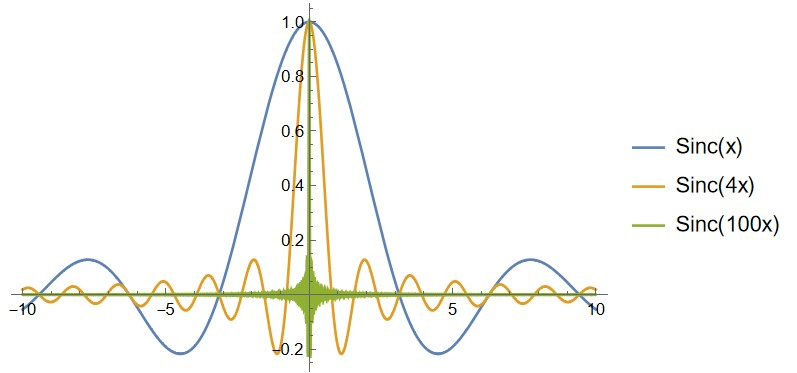
\includegraphics[width=9cm]{sinc-lim}
		\caption{plots of the cardinal sine function $\sinc(n \,t)$ for different values of $n$.} \label{fig:four:sinclim}
	\end{SCfigure}
	As shown in figure \ref{fig:four:sinclim} pushing the limit for the sine function results in a \textit{Dirac's delta distribution-like} function.
	
	\paragraph{Duality principle} Confronting results of equation \ref{eq:four:impulsetransf} and \ref{eq:four:consttransform} we can see that there's a sort of \textit{dual representation}: the transform of a pulse is a unitary signal in the frequency domain while a constant function in the time domain is transformed into a pulse in the frequency domain. This idea is generalized by the \de{duality principle} stating that
	\begin{align*}
		\textrm{if } & X(\Omega) = \four{x(t)} \\
		\textrm{then }& \four{X(t)} = x(-\Omega) \quad \textrm{and} \quad \four{x(\Omega)} = X(-t)
	\end{align*}
	
	\paragraph{Harmonics functions} Considering the case of a generic co-sinusoidal of amplitude $A$, pulsation $\Omega_0$ and initial phase $\phi_0$ determining the signal $x(t) = A \cos(\Omega_0t+\phi_0)$. Applying the definition of the \ctft we determine the spectrum
	\begin{equation}
	\begin{aligned}
		\four{A \cos\big(\Omega_0 t + \phi_0\big)} & = \intinf A  \cos\big(\Omega_0 t + \phi_0\big) e^{-j\Omega t} \, dt \\ 
		& = \intinf A \left( \frac{e^{j(\phi_0 + \Omega_0 t)} + e^{-j(\phi_0 - \Omega_0t)} }{2} \right) e^{-j\Omega t}\, dt \\
		& = \frac A 2 e^{j\phi_0} \lim_{\tau\rightarrow\infty} \int_{-\tau}^\tau e^{j(\Omega_0-\Omega)t}\, dt + \frac A 2 e^{-j\phi_0} \lim_{\tau\rightarrow\infty} \int_{-\tau}^\tau e^{-j(\Omega_0-\Omega)t}\, dt \\
		& = \frac A 2 e^{j\phi_0} \lim_{\tau\rightarrow\infty} 2\tau \sinc\Big(\big(\Omega-\Omega_0\big)t\Big) + \frac A 2 e^{-j\phi_0} \lim_{\tau\rightarrow\infty} 2\tau \sinc\Big(\big(\Omega-\Omega_0\big)t\Big) \\
		& = \frac A 2 e^{j\phi_0} \delta\big(\Omega - \Omega_0\big) + \frac A 2 e^{-j\phi_0} \delta\big(\Omega + \Omega_0\big)
	\end{aligned}
	\end{equation}
	\begin{note}
		to prove such relation the complex notation of the cosine has been used, in fact
		\[ \cos x = \frac{e^{jx} + e^{-jx}}{2} \hspace{3cm} \sin x = \frac{e^{jx} - e^{-jx}}{2} \]
	\end{note} \noindent
	Similarly it can be proven that
	\[ \four{A \sin(\Omega_0 t + \phi_0)} = \frac A {2j} e^{j\phi_0} \delta\big(\Omega - \Omega_0\big) - \frac A {2j} e^{-j\phi_0} \delta\big(\Omega + \Omega_0\big) \]
	
	From this expressions we can see that the transform of sinusoidal functions are described by pulses in the complex frequency domain; in particular the magnitude present Dirac's delta function of amplitude $\frac A 2$ at the frequencies $\pm \Omega_0$ and with a phase depending on $\phi_0$.
	
	\paragraph{Periodic signals} Considering now periodic signals of period $T$, using the Fourier series they can be decomposed into a sum of harmonic signals of the form
	\[ x(t) = \frac{a_0}{2} + \sum_{m=1}^\infty a_m \cos\left( \frac{2\pi m}{T} t \right) + \sum_{m=1}^\infty b_m \sin\left( \frac{2\pi m}{T} t \right) \]
	Applying the yet proven transform of (cos)sinusoidal function then the spectrum of a periodic signal can be regarded as the a sequence of Dirac pulses in the frequency domain in the form:
	\begin{equation}
		X(\Omega) = \frac{a_0}{2} \delta(\Omega) + \sum_{m=1}^{\infty} \frac{a_m - j b_m}{2} \left[ \delta\left( \delta \left( \Omega - \frac{2\pi m}{T}\right) \right) - \delta\left( \Omega + \frac{2\pi m}{T} \right) \right]
	\end{equation}

	\paragraph{Exponential} Let's consider the signal $x(t)$ defined as a exponential only for the positive time range, and so of the form $x(t) = e^{-\alpha t} u(t)$ (where $u(t)$ is the \textit{unit step} that's 1 for $t\geq 0$ and 0 for $t<0$). Considering the sufficient condition described at page \pageref{sec:four:sufficient}, the signal $x(t)$ in order to be transformable needs to have a energy that doesn't diverge: such criteria is matched every time $\alpha >0$. With this assumption the associated transform can be computed as
	\begin{equation}
	\begin{aligned}
		X(\Omega) & = \intinf e^{-\alpha t} u(t) e^{-j\Omega t}\, dt = \int_0 ^\infty e^{-(\alpha + j\Omega) t} \, dt = - \frac{1}{\alpha + j\Omega} e^{-(\alpha + j\Omega) t} \Big|_0^\infty \\
		& = \frac{1}{\alpha + j\Omega}
	\end{aligned}
	\end{equation}
	
	\paragraph{Unit step} Considering the unit step function $u(t)$ defined as
	\begin{equation}
		u(t) = \begin{cases}
			1 \qquad & t\geq0 \\ 0 & t < 0
		\end{cases}
	\end{equation}
	then such function can also be rewritten as the sum of other 2 functions $u_1,u_2$ in the form
	\[ u(t) = u_1(t) + u_2(t) = \frac 1 2 +\frac 1 2 \textrm{sign} (t) \qquad \textrm{where } \textrm{sign(t)} = \lim_{\alpha\rightarrow 0} \begin{cases}
		e^{-\alpha|t|} \qquad &t\geq 0\\
		-e^{-\alpha|t|} \qquad &t< 0\\
	\end{cases} \]
	Using the linear property of the Fourier transform the spectrum $U$ can be regarded as the sum of the spectrum of the constant term $u_1$ (that's $\frac 1 2 \delta(\Omega)$) while the transform of $u_2$ can be regarded as
	\[ U_2(\Omega) = \frac 1 2 \lim_{\alpha\rightarrow0} \left( \frac{1}{a+j\Omega} - \frac{1}{\alpha - j \Omega} \right) = -\frac 1 2 \lim_{\alpha\rightarrow0} \frac{2j\Omega}{\alpha^2+\Omega^2} \]
	Combining the two results we so have that
	\begin{equation}
		U(\Omega) = U_1(\Omega) + U_2(\Omega) = \frac 1 2\delta(\Omega) + \frac{1}{j\Omega}
	\end{equation}
	
	
\subsection{Discrete time}		
	\paragraph{Kronecker pulse} The Kronecker pulse $\delta(n)$ is the discrete-time analogous of the the Dirac's delta distribution and is defined as
	\begin{equation}
		\delta (n) = \begin{cases}
			1 \qquad & n = 0 \\ 0 & n\neq0
		\end{cases}
	\end{equation}
	Similarly to the continuous-time case, it's \dtft it's equal to
	\begin{equation}
	\begin{aligned}
		\four{\delta(n)} & = \infsum n \delta(n) e^{-j\omega n} = e^{-j\omega 0} = 1 \\
		\four{\delta(n-n_0)} & = e^{-j\omega n_0}
	\end{aligned} \hspace{2cm} \forall \omega
	\end{equation}
	where the transform of the shifted pulse is computed considering the related property.
	
	\paragraph{Constant signal} Considering the unitary constant signal $x(n) = 1$ for all $n$ (every constant can be obtained as multiplication of such signal) that can so be described as a \textit{train of Kronecker pulses} in the form
	\[  x(t) = \infsum k \delta(n-k)  \]
	then so it's \dtft can be regarded as
	\begin{equation}
		X\big(e^{j\omega}\big) = 2 \pi \infsum k \delta\big(\omega - 2\pi k)
	\end{equation}
	
	\paragraph{Converging exponential sequence} Considering the case of the exponential sequence $x(n) = a^n u(n)$ only for positive values of $n$, in order to have an absolutely convergent series we must ensure to have $|a|< 1$. With that assumption the \dtft can be computed as
	\[ X\big(e^{j\omega}\big) = \sum_{n=0}^\infty a^n e^{-j\omega n} = \sum_{n=0}^\infty \big(a e^{-j\omega}\big)^n \]
	Considering $a e^{-j\omega} = b$ then this expression can be seen as a convergent geometric series and so
	\begin{equation}
		X\big(e^{j\omega}\big) = \lim_{N\rightarrow \infty} \sum_{n=0}^N b^n = \lim_{N\rightarrow 0} \frac{1-b^{N+1}}{1-b} = \frac 1 {1-b} = \frac{1}{1-ae^{-j\omega}}
	\end{equation}
	\begin{note} \label{sec:four:geometricalprogression}
		Given a geometric series $a_n = q a_{n-1}$ it can be proven that, if $|q| < 1$, the sum of the first $N$ terms is
		\[ \sum_{n=1}^N a_n = \frac{1-q^N}{1-q} \]
	\end{note}
	
	
	
	
	
	